\documentclass[11pt, oneside, a4paper]{article}

%--- PREAMBLE ---%
\usepackage{geometry}
\usepackage[utf8]{inputenc}
\usepackage[T1]{fontenc}
\usepackage{hyperref}
\usepackage{float}
\usepackage{amsmath}
\usepackage{amssymb}
\usepackage{pgfplots}
\pgfplotsset{width=10cm,compat=1.9}

\setcounter{tocdepth}{2}
\hypersetup{
	hidelinks
}

\title{CMPE 300: Project 1}
\author{
	Buğra Keser\\2021400144
	\and
	Yusuf Anıl Yazıcı\\2021400207
}
\date{November 17, 2024}

%-- DOCUMENT ---%

\begin{document}
	\maketitle

	\tableofcontents

	\newpage

	\section{Theoretical Analysis}


\subsection{Basic operation is the comparison marked as (1)}
Assuming that the comparison marked as (1) is the basic operation, the number of basic operations remains the same for all cases, as the comparison is executed with every increment in the for loop, regardless of any other operations and input types.

\subsubsection{Analysis of B(n)}
As the for loop executes \( n \) times, the comparison is also executed \( n \) times. Therefore, the number of basic operations is \( n \) ,which implies asymptotic notation of $\theta(n)$.
\[
B(n) = n \in \boldsymbol{\theta(n)}
\]

\subsubsection{Analysis of W(n)}
As the for loop executes \( n \) times, the comparison is also executed \( n \) times. Therefore, the number of basic operations is \( n \), which implies asymptotic notation of $\theta(n)$.
\[
W(n) = n \in \boldsymbol{\theta(n)}
\]

\subsubsection{Analysis of A(n)}
As the for loop executes \( n \) times, the comparison is also executed \( n \) times. Therefore, the number of basic operations is \( n \), which implies asymptotic notation of $\theta(n)$.
\[
A(n) = n \in \boldsymbol{\theta(n)}
\]


	\subsection{Basic operations are the two loop increments marked as (2)}

	\subsubsection{Analysis of B(n)}
The best case for the input occurs when all elements of the array are either 'm' or 'p', as the marked basic operations are never executed. This is because the corresponding \texttt{if} conditions that trigger the execution of the marked operations are never satisfied. Thus, the number of basic operations for such an input is 0, which implies asymptotic notation of $O(1)$.

\[
B(n) = 0 \in \boldsymbol{O(1)}
\]

	\subsubsection{Analysis of W(n)}
 
The worst-case scenario occurs when the array consists only of 'c' letters, as this triggers the execution of the basic operation based on the input size each time, unlike the 'e' case, which depends on the index of the letter. This ensures that the basic operation is executed more frequently.

The y-value of the inner for loop jumps \( j \) times—which depends on the value of \( i \) in the outer loop—every time it is iterated, yielding the following equation: \(( n +  \sum_{i=1}^{n} \lfloor\frac{n}{i} \rfloor)\).


\begin{flushleft}
Taking into account the outer loop, which executes n times, the notation for the analysis is as follows:
\[
n \cdot \left( n +  \sum_{i=1}^{n} \lfloor \frac{n}{i} \rfloor \right)
\]
\end{flushleft}
The summation notation \(\sum_{i=1}^{n} \lfloor \frac{n}{i} \rfloor\) yields \(\theta(n \log n)\) due to the harmonic series' behavior when summed over all \( i \). Since this term is multiplied by \( n \) in the final expression \( n \cdot \left( n + \sum_{i=1}^{n} \lfloor \frac{n}{i} \rfloor \right) \), the resulting time complexity becomes \(\theta(n^2 \log n)\). This is because multiplying \(\theta(n \log n)\) by \( n \) scales the complexity to $\theta(n^2 \log n)$.


\[
W(n) = n \cdot \left( n +  \sum_{i=1}^{n} \lfloor \frac{n}{i} \rfloor \right) \in \boldsymbol{\theta(n^2 \log n)}
\]


	\subsubsection{Analysis of A(n)}
 The average case analysis requires considering the probability distribution of the different input elements ('c', 'm', 'p', 'e') and the number of times the basic operations are executed for each scenario. Let's divide the analysis into steps and clearly analyze the conditional probabilities.

\[
A(n) = \mathbb{E}[T] = \mathbb{E}[T_1] + \mathbb{E}[T_2] + \mathbb{E}[T_3]
\]

 where $T_1$ is the number of basic operations involved when the if condition matches 'c', $T_2$ is the number of basic operations involved when the if condition matches either 'm' or 'p' and $T_3$ is the number of basic operations involved when the if condition matches 'e'.

\textbf{1. $\mathbf{E[T_1]}$}:
 The occurrence of the letter 'c' in a n-size array is n/8 on average as the probability suggests. The expression in the parentheses is analyzed for the worst-case scenario, the difference is only the number of 'c' letters. This is handled by dividing the size by eight giving the expression below:
   \[
   \frac{n}{8} \cdot \left( n +  \sum_{i=1}^{n} \lfloor \frac{n}{i} \rfloor \right)\]
   

\textbf{2. $\mathbf{E[T_2]}$}:
In the if blocks that check whether the element of the array is 'm' or 'p', no basic operations are performed, as these code blocks do not contain any basic operation. Thus, the equation is as follows:
   \[\frac{n}{4} \cdot 0 + \frac{n}{8} \cdot 0 \]
   These terms do not contribute to the basic operations as they yield 0.

\textbf{3. $\mathbf{E[T_3]}$}:
\[
\mathbb{E}[T_3] = \sum_{i=0}^{n-1} \mathbb{E}[\tau \mid X=i] \cdot P(X=i)
\]
Here the X is the index of the 'c' letter, so $\mathbb{E}[\tau \mid X=i]$ = i and P(X=i) = 1/2 as it is given.
Then, such an expression is obtained \[\mathbb{E}[T_3] = \sum_{i=0}^{n-1} \frac{i}{2} = \frac{n(n-1)}{4} = \frac{(n^2 - n)}{4}\]

Combining these steps:
\begin{equation*}
A(n) = \frac{3n^2}{8} - \frac{n}{4} + \frac{n}{8} \cdot  \sum_{i=1}^{n} \lfloor \frac{n}{i} \rfloor 
\end{equation*}

In the right-most term, the summation notation \(\sum_{i=1}^{n} \lfloor \frac{n}{i} \rfloor\) yields \(\theta(n \log n)\) due to the harmonic series' behavior when summed over all \( i \). With the multiplication of the notation by n/8, the time complexity of the term results in \(\theta(n^2 \log n)\). That makes this term the most dominant one as n grows. Theta analysis is:



\[
A(n) = \frac{3n^2}{8} - \frac{n}{4} + \frac{n}{8} \cdot  \sum_{i=1}^{n} \lfloor \frac{n}{i} \rfloor  \in \boldsymbol{\theta(n^2 \log n)}
\]





	\subsection{Basic operations are the four assignments marked as (3)}

\subsubsection{Analysis of B(n)}

The best-case scenario for the input occurs when the first element is 'e' and the remaining elements are 'p'. When the first element is 'e', no basic operations are executed since the condition for the outer loop is not satisfied. In the case of 'p', the number of basic operations is determined by taking the floor of the array size divided by 5 continuously giving the logarithmic term. The expression is:
\begin{equation*}
0 + (n-1) \cdot \left( \lfloor \log_5 n \rfloor + 1 \right)
\end{equation*}

For larger inputs, \( (n-1) \) term behaves like \( n \) and the other term behaves like \( \log n \), which yields the complexity of $\theta(n \log n)$.

\[
B(n) = (n-1) \cdot \left( \lfloor \log_5 n \rfloor + 1 \right) \in \boldsymbol{\theta(n \log n)}
\]


\subsubsection{Analysis of W(n)}

The worst-case scenario for the input occurs when the first element is 'c' and the remaining elements are 'e'. In the case of 'e', more basic operations are performed except for the 0th index, which has the highest number of basic operations for the 'c' case as it depends on \( n \), whereas 'e' does not involve any basic operations. For the 'c' case, the number of basic operations is determined by the size of the array, \( n \). For the remaining part, consisting of all 'e' cases, the number of basic operations is determined by three nested sigma notations, given by \( \sum_{i=0}^{n-1} \sum_{m=1}^{i} \sum_{l=m}^{n} 1 \). Summing n with the result of the nested sigma notations, the expression is as follows:


\begin{equation*}
n+ \frac{n^3 - n}{3} 
\end{equation*}

As n grows, the dominant term is $n^3$, implying the theta notation of $(\theta(n^3))$.

\[
W(n) = \frac{n^3 + 2n}{3}  \in \boldsymbol{\theta(n^3)}
\]


\subsubsection{Analysis of A(n)}

 The average case analysis requires considering the probability distribution of the different input elements ('c', 'm', 'p', 'e') and the number of times the basic operations are executed for each scenario. Let's divide the analysis into steps and clearly analyze the conditional probabilities.

 \[
A(n) = \mathbb{E}[T] = \mathbb{E}[T_1] + \mathbb{E}[T_2] + \mathbb{E}[T_3] + \mathbb{E}[T_4]
\]

 where $T_1$ is the number of basic operations involved when the if condition matches 'c', $T_2$ is the number of basic operations involved when the if condition matches 'm', $T_3$ is the number of basic operations involved when the if condition matches 'p' and $T_4$ is the number of basic operations involved when the if condition matches 'e'.


\textbf{1. $\mathbf{E[T_1]}$}:


 The occurrence of the letter 'c' in a n-size array is n/8 on average as the probability suggests. The basic operation is performed n times for each term. As the frequency of ‘c’ is n/8, the following formula is obtained:
   
   \[
   \frac{n}{8} \cdot  n \]

   

\textbf{2. $\mathbf{E[T_2]}$}:

 For each term, number of basic operation is determined by a logarithmic term in base 2, since the basic operation is performed until n is exceeded by continuous multiplication of 2. Multiplying with the average occurrence of the letter 'm' in a n-size array, that is n/4, the following expression is obtained: 
\[
\frac{n}{4} \cdot \lceil \log_2 n \rceil
\]

\textbf{3. $\mathbf{E[T_3]}$}:

For each term, the number of basic operations is determined by taking the floor of the array size divided by 5 continuously giving the logarithmic term in base 5. Multiplying with the average occurrence of the letter 'p' in a n-size array, that is n/8, the following expression is obtained: 
\[ 
\frac{n}{8} \cdot \left( \lfloor \log_5 n \rfloor + 1 \right)
\]

\textbf{4. $\mathbf{E[T_4]}$}:

\[
\mathbb{E}[T_4] = \sum_{i=0}^{n-1} \mathbb{E}[\tau \mid X=i] \cdot P(X=i)
\]
P(X = i) is 1/2 as it is given, and the $\mathbb{E}[\tau \mid X=i]$ is calculated as follows:
\[
\mathbb{E}[\tau \mid X=i] = \sum_{m=1}^{i} \sum_{l=m}^{n} 1 = ni - \frac{i^2}{2} + \frac{i}{2} 
\]

\[
\mathbb{E}[T_4] = \frac{1}{2} \sum_{i=0}^{n-1} (ni - \frac{i^2}{2} + \frac{i}{2}) = \frac{n^3 - n}{6}
\]

Combining these contributions:

\begin{equation*}
A(n) = \frac{n^3}{6} + \frac{n^2}{8} + \frac{n}{4} \cdot \lceil \log_2 n \rceil + \frac{n}{8} \cdot \lfloor \log_5 n \rfloor  - \frac{n}{24}
\end{equation*}


The dominant term here is \( \frac{n^3}{6}\) , as it grows faster than all other terms. Therefore, the final average case complexity is:

\[
A(n) = \frac{n^3}{6} + \frac{n^2}{8} + \frac{n}{4} \cdot \lceil \log_2 n \rceil + \frac{n}{8} \cdot \lfloor \log_5 n \rfloor  - \frac{n}{24} \in \boldsymbol{\theta(n^3)}
\]




	\subsection{Basic operations are the four assignments marked as (4)}

\subsubsection{Analysis of B(n)}

The best-case scenario for the input occurs when the first element is 'e' and the remaining elements are 'p'. When the first element is 'e', no basic operations are executed since the condition for the outer loop is not satisfied. In the case of 'p', the number of basic operations is determined by taking the floor of the array size divided by 5 continuously giving the logarithmic term. The expression is:
\begin{equation*}
0 + (n-1) \cdot \left( \lfloor \log_5 n \rfloor + 1 \right)
\end{equation*}

For larger inputs, \( (n-1) \) term behaves like \( n \) and the other term behaves like \( \log n \), which yields the complexity of \( \theta(n \log n) \).

\[
B(n) = (n-1) \cdot \left( \lfloor \log_5 n \rfloor + 1 \right) \in \boldsymbol{ \theta(n \log n) }
\]

	\subsubsection{Analysis of W(n)}
 The worst-case scenario for the input occurs when the first element is 'c' and the remaining elements are 'e'. In the case of 'e', more basic operations are performed except for the 0th index, which has the highest number of basic operations for the 'c' case as it depends on \( n \), whereas 'e' does not involve any basic operations. For the 'c' case, the y-value of the inner for loop jumps \( j \) times—which depends on the value of \( i \) in the outer loop—every time it is iterated, yielding the following equation: \(( n +  \sum_{i=1}^{n} \lfloor\frac{n}{i} \rfloor)\). For the remaining part, consisting of all 'e' cases, the number of basic operations is determined by three nested sigma notations. Adding up the two parts, a general expression is obtained:
\[
( n +  \sum_{i=1}^{n} \lfloor\frac{n}{i} \rfloor) +  \sum_{i=0}^{n-1} \sum_{m=1}^{i} \sum_{l=m}^{n} n
\]
 
 
 Summing these and converting nested sigma notations into the regular formula, the expression is as follows:

\begin{equation*}
\left( n +  \sum_{i=1}^{n} \lfloor\frac{n}{i} \rfloor \right) + \frac{n^4 - n^2}{3}
\end{equation*}
The harmonic series with n over all i gives the time complexity of $n \cdot\log n$ as harmonic series approaches $\log n$ as n grows.
Thus, the dominant term is $n^4$ for larger values of n, implying the theta notation of \( \theta(n^4) \).

\[
W(n) = \left( n +  \sum_{i=1}^{n} \lfloor\frac{n}{i} \rfloor \right) + \frac{n^4 - n^2}{3} \in \boldsymbol{\theta(n^4)}
\]

	
        \subsubsection{Analysis of A(n)}
The average case analysis requires considering the probability distribution of the different input elements ('c', 'm', 'p', 'e') and the number of times the basic operations are executed for each scenario. Let's divide the analysis into steps and clearly analyze the conditional probabilities.


 \[
A(n) = \mathbb{E}[T] = \mathbb{E}[T_1] + \mathbb{E}[T_2] + \mathbb{E}[T_3] + \mathbb{E}[T_4]
\]

 where $T_1$ is the number of basic operations involved when the if condition matches 'c', $T_2$ is the number of basic operations involved when the if condition matches 'm', $T_3$ is the number of basic operations involved when the if condition matches 'p' and $T_4$ is the number of basic operations involved when the if condition matches 'e'


\textbf{1. $\mathbf{E[T_1]}$}:


 The occurrence of the letter 'c' in a n-size array is n/8 on average as the probability suggests. The basic operation is performed \(( n +  \sum_{i=1}^{n} \lfloor\frac{n}{i} \rfloor)\) times for each term as explained in the worst-case analysis. As the frequency of ‘c’ is n/8, the following formula is obtained:
   
   \[
   \frac{n}{8} \cdot  ( n +  \sum_{i=1}^{n} \lfloor\frac{n}{i} \rfloor) \]

   


\textbf{2. $\mathbf{E[T_2]}$}:

 For each term, number of basic operation is determined by a logarithmic term in base 2, since the basic operation is performed until n is exceeded by continuous multiplication of 2. Multiplying with the average occurrence of the letter 'm' in a n-size array, that is n/4, the following expression is obtained: 
\[
\frac{n}{4} \cdot \lceil \log_2 n \rceil
\]

\textbf{3. $\mathbf{E[T_3]}$}:

For each term, the number of basic operations is determined by taking the floor of the array size divided by 5 continuously giving the logarithmic term in base 5. Multiplying with the average occurrence of the letter 'p' in a n-size array, that is n/8, the following expression is obtained: 
\[ 
\frac{n}{8} \cdot \left( \lfloor \log_5 n \rfloor + 1 \right)
\]

\textbf{4. $\mathbf{E[T_4]}$}:

\[
\mathbb{E}[T_4] = \sum_{i=0}^{n-1} \mathbb{E}[\tau \mid X=i] \cdot P(X=i)
\]
P(X = i) is 1/2 as it is given, and the $\mathbb{E}[\tau \mid X=i]$ is calculated as follows:
\[
\mathbb{E}[\tau \mid X=i] = \sum_{m=1}^{i} \sum_{l=m}^{n} n = n^2i - n\frac{i^2}{2} + n\frac{i}{2} 
\]

\[
\mathbb{E}[T_4] = \frac{1}{2} \sum _{i=0}^{n-1}( n^2i - n\frac{i^2}{2} + n\frac{i}{2} )= \frac{n^4 - n^2}{6}
\]

Combining these contributions:
     
\begin{equation*}
A(n) = \frac{n^4}{6} - \frac{n^2}{24} + \frac{n}{8} \cdot \sum_{i=1}^{n} \lfloor\frac{n}{i} \rfloor + \frac{n}{4} \cdot \lceil \log_2 n \rceil + \frac{n}{8} \cdot \lfloor \log_5 n \rfloor + \frac{n}{8}
\end{equation*}

The dominant term here is \( \frac{n^4}{6}\) , as it grows faster than all other terms. Therefore, the final average case complexity is:

\[
A(n) = \frac{n^4}{6} - \frac{n^2}{24} + \frac{n}{8} \cdot \sum_{i=1}^{n} \lfloor\frac{n}{i} \rfloor + \frac{n}{4} \cdot \lceil \log_2 n \rceil + \frac{n}{8} \cdot \lfloor \log_5 n \rfloor + \frac{n}{8} \in \boldsymbol{\theta(n^4)}
\]


	\section{Identification of Basic Operation(s)}
The assignments marked as (4) were chosen as basic operations because they dominate the computational workload in nested loops, directly impacting runtime. These operations reflect the critical computational steps that align with real execution time in practical scenarios.



	\section{Real Execution}

	\begin{table}[H]
		\centering
		\begin{tabular}{|l|l|} \hline
			\textbf{N Size} & \textbf{Time Elapsed (sec)} \\ \hline
			1 & \( 7.15 \times 10^{-7}\) \\ \hline
			5 & \( 1.00 \times 10^{-6}\) \\ \hline
			10 & \( 1.07 \times 10^{-6}\) \\ \hline
			20 & \( 1.98 \times 10^{-6}\) \\ \hline
			30 & \( 3.96 \times 10^{-6}\) \\ \hline
			40 & \( 4.94 \times 10^{-6}\) \\ \hline
			50 & \( 6.03 \times 10^{-6}\) \\ \hline
			60 & \( 7.30 \times 10^{-6}\) \\ \hline
			70 & \( 9.11 \times 10^{-6}\) \\ \hline
			90 & \( 1.08 \times 10^{-5}\) \\ \hline
			100 & \( 1.22 \times 10^{-5}\) \\ \hline
			120 & \( 1.45 \times 10^{-5}\) \\ \hline
			130 & \( 2.30 \times 10^{-5}\) \\ \hline
			140 & \( 2.39 \times 10^{-5}\) \\ \hline
			150 & \( 2.66 \times 10^{-5}\) \\ \hline
			160 & \( 2.80 \times 10^{-5}\) \\ \hline
			170 & \( 3.20 \times 10^{-5}\) \\ \hline
		\end{tabular}
		\caption{Best Case Real Execution Times}
		\label{tab:best-case}
	\end{table}


	\begin{table}[H]
		\centering
		\begin{tabular}{|l|l|} \hline
			\textbf{N Size} & \textbf{Time Elapsed (sec)} \\ \hline
			1 & \( 5.72 \times 10^{-7}\) \\ \hline
			5 & \( 7.72 \times 10^{-6}\) \\ \hline
			10 & \( 8.43 \times 10^{-5}\) \\ \hline
			20 & \( 1.33 \times 10^{-3}\) \\ \hline
			30 & \( 6.52 \times 10^{-3}\) \\ \hline
			40 & \( 2.01 \times 10^{-2}\) \\ \hline
			50 & \( 4.80 \times 10^{-2}\) \\ \hline
			60 & \( 9.83 \times 10^{-2}\) \\ \hline
			70 & \( 1.85 \times 10^{-1}\) \\ \hline
			90 & \( 5.01 \times 10^{-1}\) \\ \hline
			100 & \( 7.55 \times 10^{-1}\) \\ \hline
			120 & \( 1.54 \) \\ \hline
			130 & \( 2.11 \) \\ \hline
			140 & \( 2.84 \) \\ \hline
			150 & \( 3.74 \) \\ \hline
			160 & \( 4.82 \) \\ \hline
			170 & \( 6.12 \) \\ \hline
		\end{tabular}
		\caption{Worst Case Real Execution Times}
		\label{tab:worst-case}
	\end{table}

	\begin{table}[H]
		\centering
		\begin{tabular}{|l|l|} \hline
			\textbf{N Size} & \textbf{Time Elapsed (sec)} \\ \hline
			1 & \( 5.96 \times 10^{-7}\) \\ \hline
			5 & \( 5.53 \times 10^{-6}\) \\ \hline
			10 & \( 5.39 \times 10^{-5}\) \\ \hline
			20 & \( 7.34 \times 10^{-4}\) \\ \hline
			30 & \( 3.45 \times 10^{-3}\) \\ \hline
			40 & \( 9.99 \times 10^{-3}\) \\ \hline
			50 & \( 2.88 \times 10^{-2}\) \\ \hline
			60 & \( 5.49 \times 10^{-2}\) \\ \hline
			70 & \( 1.32 \times 10^{-1}\) \\ \hline
			90 & \( 2.54 \times 10^{-1}\) \\ \hline
			100 & \( 4.06 \times 10^{-1}\) \\ \hline
			120 & \( 8.01 \times 10^{-1}\) \\ \hline
			130 & \( 1.13 \) \\ \hline
			140 & \( 1.46 \) \\ \hline
			150 & \( 2.01 \) \\ \hline
			160 & \( 2.53 \) \\ \hline
			170 & \( 3.26 \) \\ \hline
		\end{tabular}
		\caption{Average Case Real Execution Times}
		\label{tab:avg-case}
	\end{table}

	\section{Comparison}

	\subsection{Best Case}

	\subsubsection{Graph of the real execution time of the algorithm}

	% Here is an example line plot of data points for you. Feel free to change it or use something else.

	\begin{figure}[H]
	\centering
	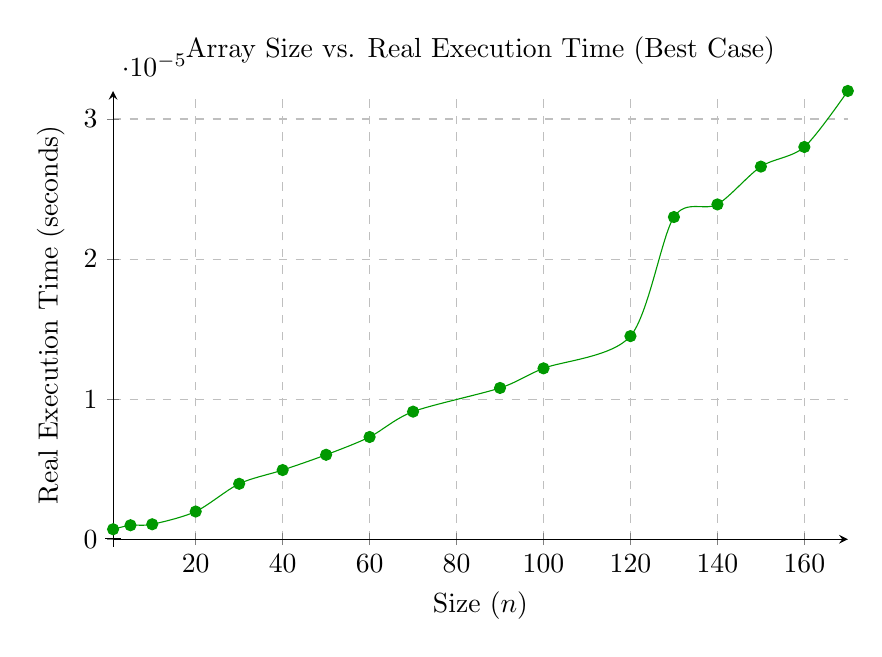
\begin{tikzpicture}
		\begin{axis}[
			% Axis labels and title
			title={Array Size vs. Real Execution Time (Best Case)},
			xlabel={Size (\(n\))},
			ylabel={Real Execution Time (seconds)},
			% Axis limits
			%xmin=0, xmax=100,
			ymin=0, %ymax=200,
			% Axis ticks
			% xtick={0,20,40,60,80,100},
			% ytick={0,20,40,60,80,100,120},
			grid=both,
			axis lines=left,
			axis line style={|-stealth},
			grid style=dashed,
			width=0.9\textwidth,
			height=\axisdefaultheight
			]
			\addplot[
				color=green!60!black,
				mark=*,
				smooth
				]
			% Change the coordinates here with your own data:
			coordinates {
				(1, 0.000000715)
				(5,   0.00000100)
				(10,  0.00000107)
				(20,  0.00000198)
				(30,  0.00000396)
				(40,  0.00000494)
				(50,  0.00000603)
				(60,  0.00000730)
				(70,  0.00000911)
				(90,  0.0000108)
				(100, 0.0000122)
				(120, 0.0000145)
				(130, 0.0000230)
				(140, 0.0000239)
				(150, 0.0000266)
				(160, 0.0000280)
				(170, 0.0000320)
			};
		\end{axis}
	\end{tikzpicture}
	\end{figure}

	\subsubsection{Graph of the theoretical analysis when basic operation is the operation marked as (1)}

    \begin{figure}[H]
	\centering
	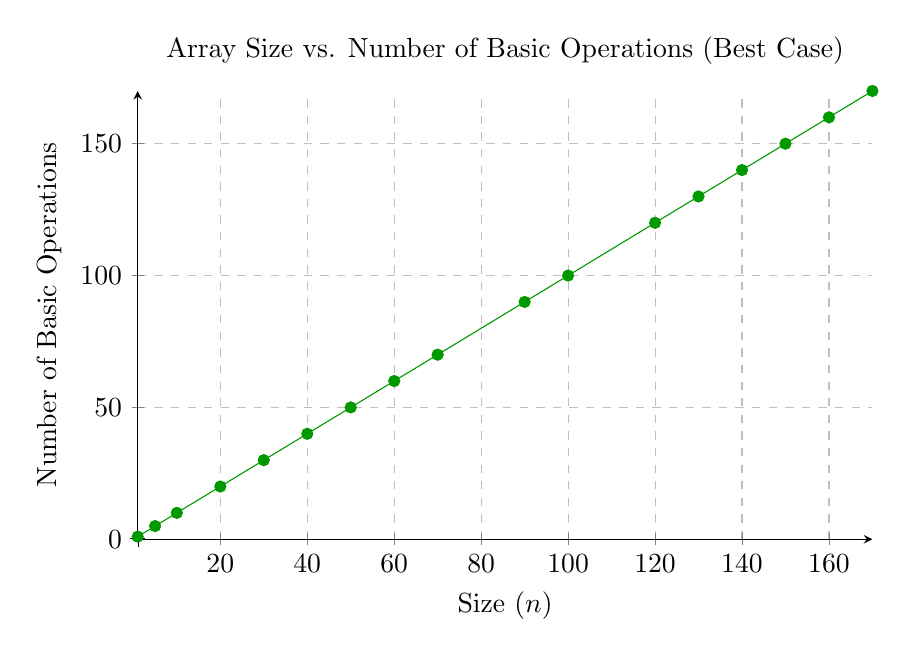
\begin{tikzpicture}
		\begin{axis}[
			% Axis labels and title
			title={Array Size vs. Number of Basic Operations (Best Case)},
			xlabel={Size (\(n\))},
			ylabel={Number of Basic Operations},
			% Axis limits
			%xmin=0, xmax=100,
			ymin=0, %ymax=200,
			% Axis ticks
			% xtick={0,20,40,60,80,100},
			% ytick={0,20,40,60,80,100,120},
			grid=both,
			axis lines=left,
			axis line style={|-stealth},
			grid style=dashed,
			width=0.9\textwidth,
			height=\axisdefaultheight
			]
			\addplot[
				color=green!60!black,
				mark=*,
				smooth
				]
			% Change the coordinates here with your own data:
			coordinates {
				(1,   1)
				(5,   5)
				(10,  10)
				(20, 20)
				(30,  30)
				(40, 40)
				(50,  50)
				(60,  60)
				(70,  70)
				(90,  90)
				(100,100)
				(120, 120)
				(130, 130)
				(140, 140)
				(150, 150)
				(160, 160)
				(170,170)
			};
		\end{axis}
	\end{tikzpicture}
	\end{figure}

	\subsubsection{Graph of the theoretical analysis when basic operation is the operation marked as (2)}

 \begin{figure}[H]
	\centering
	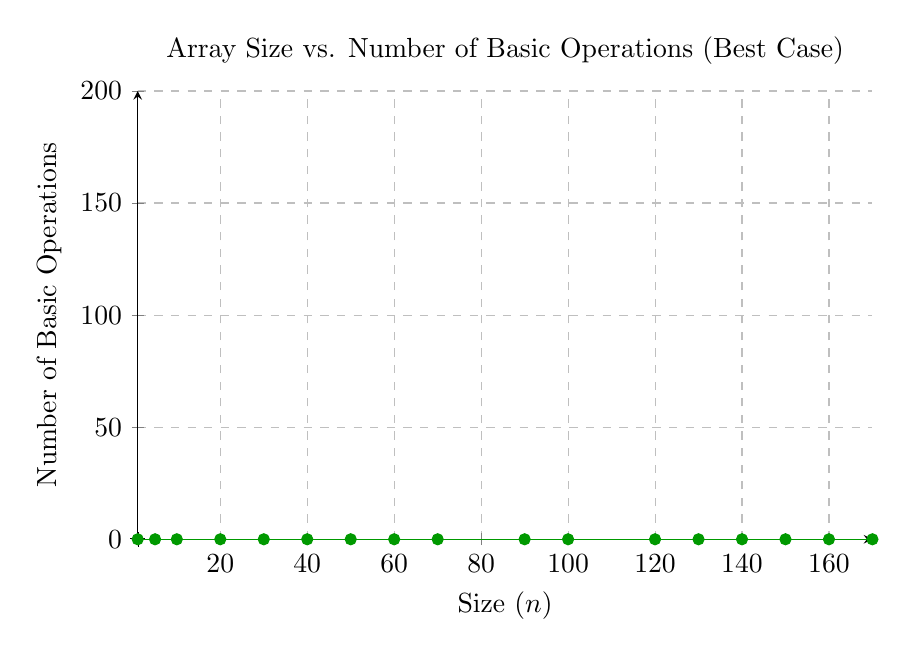
\begin{tikzpicture}
		\begin{axis}[
			% Axis labels and title
			title={Array Size vs. Number of Basic Operations (Best Case)},
			xlabel={Size (\(n\))},
			ylabel={Number of Basic Operations},
			%Axis limits
			%xmin=0, xmax=100,
		    ymin=0, ymax=200,
			% Axis ticks
			% xtick={0,20,40,60,80,100},
			% ytick={0,20,40,60,80,100,120},
			grid=both,
			axis lines=left,
			axis line style={|-stealth},
			grid style=dashed,
			width=0.9\textwidth,
			height=\axisdefaultheight
			]
			\addplot[
				color=green!60!black,
				mark=*,
				smooth
				]
			% Change the coordinates here with your own data:
			coordinates {
				(1,   0)
				(5,   0)
				(10,  0)
				(20, 0)
				(30,  0)
				(40, 0)
				(50,  0)
				(60,  0)
				(70,  0)
				(90,  0)
				(100,0)
				(120, 0)
				(130, 0)
				(140, 0)
				(150, 0)
				(160, 0)
				(170,0)
			};
		\end{axis}
	\end{tikzpicture}
	\end{figure}

	\subsubsection{Graph of the theoretical analysis when basic operation is the operation marked as (3)}

 \begin{figure}[H]
	\centering
	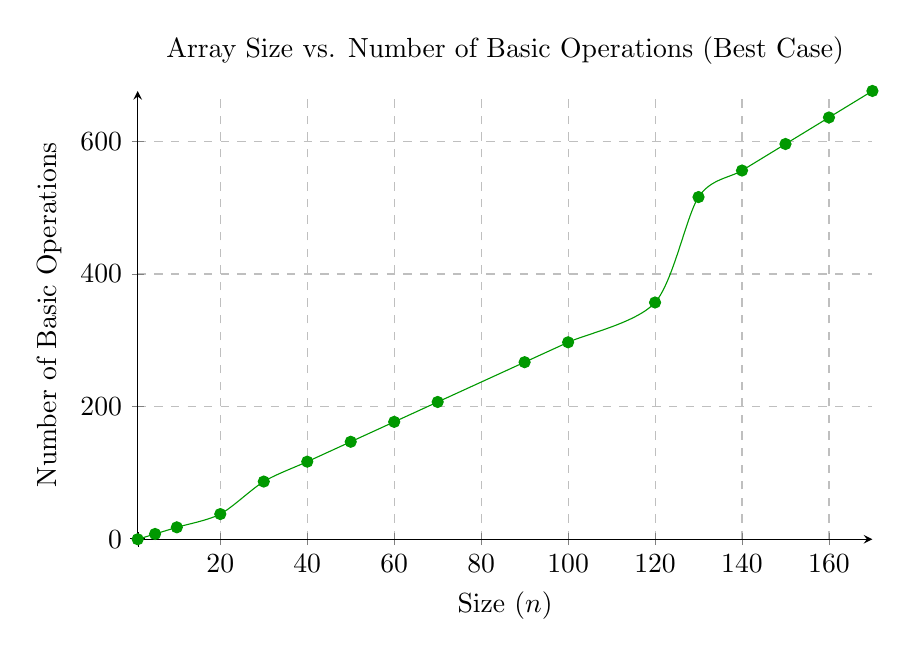
\begin{tikzpicture}
		\begin{axis}[
			% Axis labels and title
			title={Array Size vs. Number of Basic Operations (Best Case)},
			xlabel={Size (\(n\))},
			ylabel={Number of Basic Operations},
			% Axis limits
			%xmin=0, xmax=100,
			ymin=0, %ymax=200,
			% Axis ticks
			% xtick={0,20,40,60,80,100},
			% ytick={0,20,40,60,80,100,120},
			grid=both,
			axis lines=left,
			axis line style={|-stealth},
			grid style=dashed,
			width=0.9\textwidth,
			height=\axisdefaultheight
			]
			\addplot[
				color=green!60!black,
				mark=*,
				smooth
				]
			% Change the coordinates here with your own data:
			coordinates {
				(1, 0  )
				(5,  8 )
				(10, 18  )
				(20, 38)
				(30, 87 )
				(40,117 )
				(50, 147 )
				(60, 177 )
				(70, 207 )
				(90, 267 )
				(100,297)
				(120,357)
				(130, 516)
				(140,556 )
				(150, 596)
				(160,636 )
				(170,676)
			};
		\end{axis}
	\end{tikzpicture}
	\end{figure}

	\subsubsection{Graph of the theoretical analysis when basic operation is the operation marked as (4)}

 \begin{figure}[H]
	\centering
	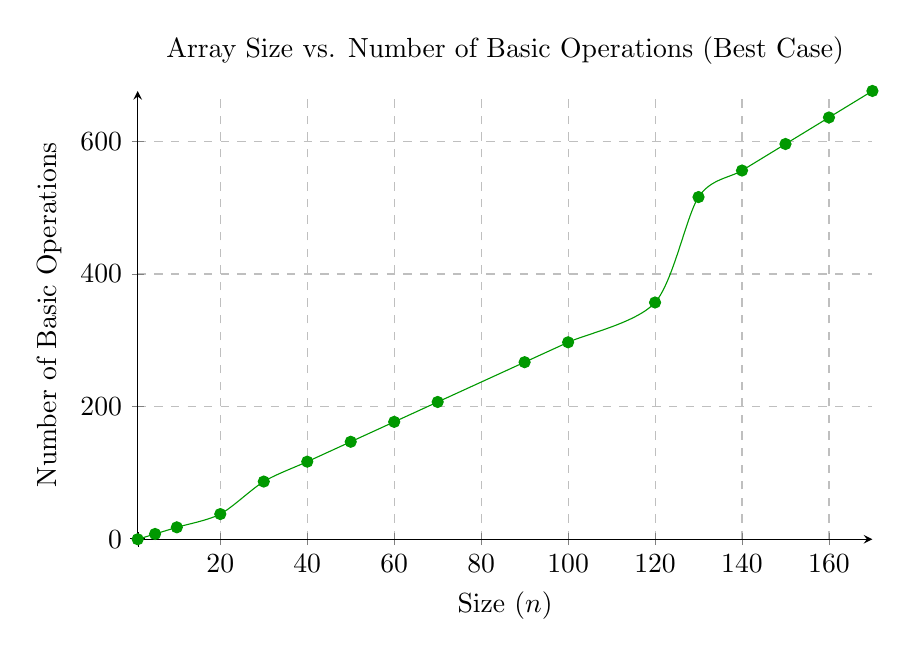
\begin{tikzpicture}
		\begin{axis}[
			% Axis labels and title
			title={Array Size vs. Number of Basic Operations (Best Case)},
			xlabel={Size (\(n\))},
			ylabel={Number of Basic Operations},
			% Axis limits
			%xmin=0, xmax=100,
			ymin=0, %ymax=200,
			% Axis ticks
			% xtick={0,20,40,60,80,100},
			% ytick={0,20,40,60,80,100,120},
			grid=both,
			axis lines=left,
			axis line style={|-stealth},
			grid style=dashed,
			width=0.9\textwidth,
			height=\axisdefaultheight
			]
			\addplot[
				color=green!60!black,
				mark=*,
				smooth
				]
			% Change the coordinates here with your own data:
			coordinates {
				(1, 0  )
				(5,  8 )
				(10, 18  )
				(20, 38)
				(30, 87 )
				(40,117 )
				(50, 147 )
				(60, 177 )
				(70, 207 )
				(90, 267 )
				(100,297)
				(120,357)
				(130, 516)
				(140,556 )
				(150, 596)
				(160,636 )
				(170,676)
			};
		\end{axis}
	\end{tikzpicture}
	\end{figure}


	\subsubsection{Comments}

    \begin{itemize}
    \item \textbf{Basic Operation Marked as (1) vs Real Execution Time:} \\
    The theoretical graph for (1) shows a linear relationship with \(n\), which does not align with the real execution graph. It fails to represent the actual computational effort of the algorithm.

    \item \textbf{Basic Operation Marked as (2) vs Real Execution Time:} \\
    The theoretical graph for (2) remains constant at zero, making it completely unrealistic and unrelated to the real execution time. This choice is invalid.

    \item \textbf{Basic Operation Marked as (3) vs Real Execution Time:} \\
    The theoretical graph for (3) reflects an \(n \log n\) growth, aligning closely with the real execution graph. This makes (3) an appropriate choice for representing the algorithm’s computational workload for the best case.

    \item \textbf{Basic Operation Marked as (4) vs Real Execution Time:} \\
    The theoretical graph for (4) reflects an \(n \log n\) growth, aligning closely with the real execution graph. This makes (4) an appropriate choice for representing the algorithm’s computational workload for the best case.
\end{itemize}




	\subsection{Worst Case}

	\subsubsection{Graph of the real execution time of the algorithm}

 \begin{figure}[H]
	\centering
	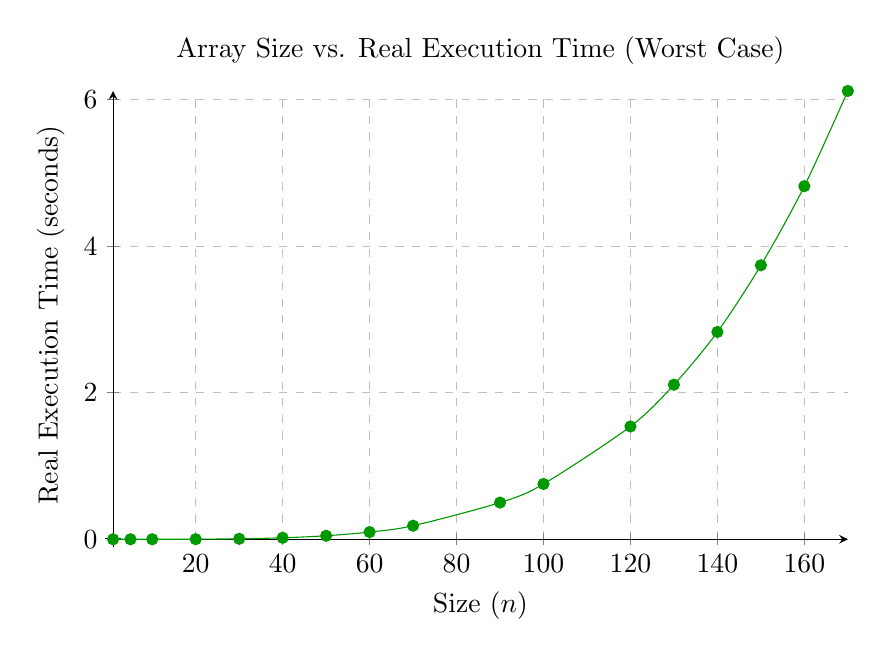
\begin{tikzpicture}
		\begin{axis}[
			% Axis labels and title
			title={Array Size vs. Real Execution Time (Worst Case)},
			xlabel={Size (\(n\))},
			ylabel={Real Execution Time (seconds)},
			% Axis limits
			%xmin=0, xmax=100,
			ymin=0, %ymax=200,
			% Axis ticks
			% xtick={0,20,40,60,80,100},
			% ytick={0,20,40,60,80,100,120},
			grid=both,
			axis lines=left,
			axis line style={|-stealth},
			grid style=dashed,
			width=0.9\textwidth,
			height=\axisdefaultheight
			]
			\addplot[
				color=green!60!black,
				mark=*,
				smooth
				]
			% Change the coordinates here with your own data:
			coordinates {
				(1,   0.000000572)
				(5,   0.00000772)
				(10,  0.0000843)
				(20,  0.00133)
				(30,  0.00652)
				(40,  0.0201)
				(50,  0.0480)
				(60,  0.0983)
				(70,  0.185)
				(90,  0.501)
				(100, 0.755)
				(120, 1.54)
				(130, 2.11)
				(140, 2.83)
				(150, 3.74)
				(160, 4.82)
				(170, 6.12)
			};
		\end{axis}
	\end{tikzpicture}
	\end{figure}

	\subsubsection{Graph of the theoretical analysis when basic operation is the operation marked as (1)}

  \begin{figure}[H]
	\centering
	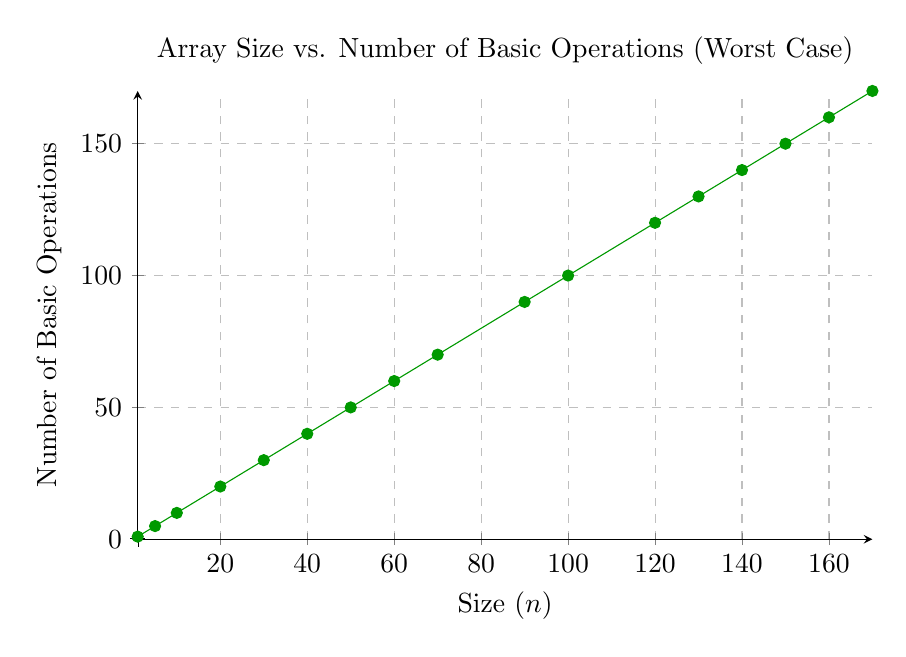
\begin{tikzpicture}
		\begin{axis}[
			% Axis labels and title
			title={Array Size vs. Number of Basic Operations (Worst Case)},
			xlabel={Size (\(n\))},
			ylabel={Number of Basic Operations},
			% Axis limits
			%xmin=0, xmax=100,
			ymin=0, %ymax=200,
			% Axis ticks
			% xtick={0,20,40,60,80,100},
			% ytick={0,20,40,60,80,100,120},
			grid=both,
			axis lines=left,
			axis line style={|-stealth},
			grid style=dashed,
			width=0.9\textwidth,
			height=\axisdefaultheight
			]
			\addplot[
				color=green!60!black,
				mark=*,
				smooth
				]
			% Change the coordinates here with your own data:
			coordinates {
				(1,   1)
				(5,   5)
				(10,  10)
				(20, 20)
				(30,  30)
				(40, 40)
				(50,  50)
				(60,  60)
				(70,  70)
				(90,  90)
				(100,100)
				(120, 120)
				(130, 130)
				(140, 140)
				(150, 150)
				(160, 160)
				(170,170)
			};
		\end{axis}
	\end{tikzpicture}
	\end{figure}

	\subsubsection{Graph of the theoretical analysis when basic operation is the operation marked as (2)}

 \begin{figure}[H]
	\centering
	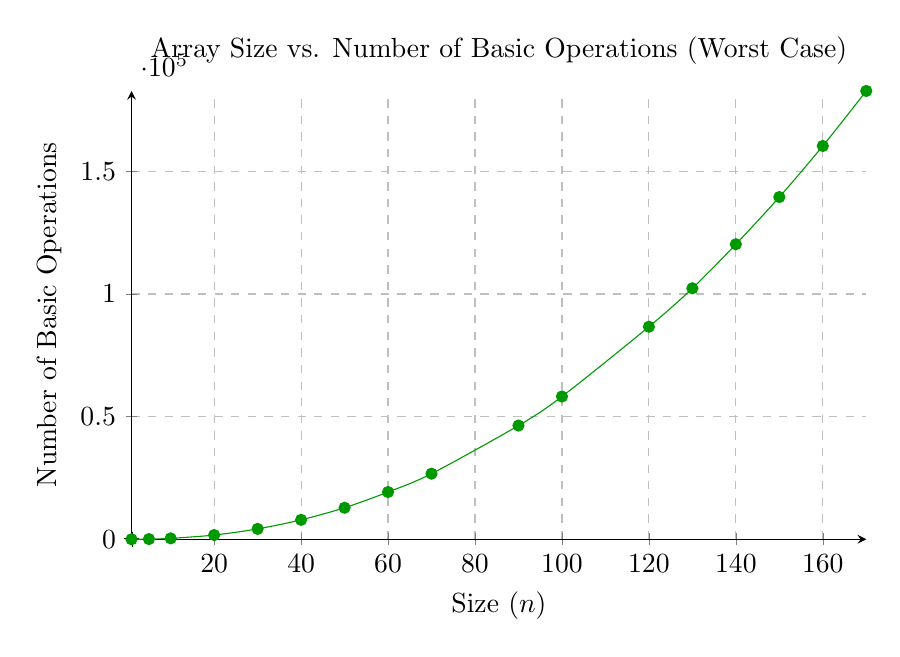
\begin{tikzpicture}
		\begin{axis}[
			% Axis labels and title
			title={Array Size vs. Number of Basic Operations (Worst Case)},
			xlabel={Size (\(n\))},
			ylabel={Number of Basic Operations},
			% Axis limits
			%xmin=0, xmax=100,
			ymin=0, %ymax=200,
			% Axis ticks
			% xtick={0,20,40,60,80,100},
			% ytick={0,20,40,60,80,100,120},
			grid=both,
			axis lines=left,
			axis line style={|-stealth},
			grid style=dashed,
			width=0.9\textwidth,
			height=\axisdefaultheight
			]
			\addplot[
				color=green!60!black,
				mark=*,
				smooth
				]
			% Change the coordinates here with your own data:
			coordinates {
				(1,   2)
				(5,   75)
				(10,  370)
				(20, 1720)
				(30,  4230)
				(40, 7920)
				(50,  12850)
				(60,  19260)
				(70,  26740)
				(90,  46350)
				(100,58200)
				(120, 86640)
				(130, 102310)
				(140, 120260)
				(150, 139500)
				(160, 160320)
				(170,182750)
			};
		\end{axis}
	\end{tikzpicture}
	\end{figure}

	\subsubsection{Graph of the theoretical analysis when basic operation is the operation marked as (3)}

 \begin{figure}[H]
	\centering
	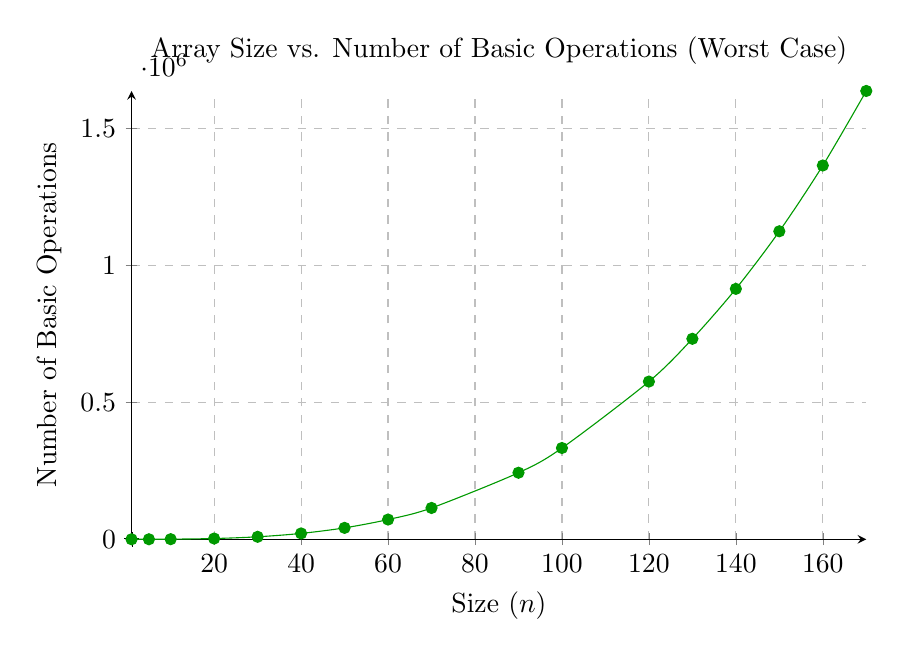
\begin{tikzpicture}
		\begin{axis}[
			% Axis labels and title
			title={Array Size vs. Number of Basic Operations (Worst Case)},
			xlabel={Size (\(n\))},
			ylabel={Number of Basic Operations},
			% Axis limits
			%xmin=0, xmax=100,
			ymin=0, %ymax=200,
			% Axis ticks
			% xtick={0,20,40,60,80,100},
			% ytick={0,20,40,60,80,100,120},
			grid=both,
			axis lines=left,
			axis line style={|-stealth},
			grid style=dashed,
			width=0.9\textwidth,
			height=\axisdefaultheight
			]
			\addplot[
				color=green!60!black,
				mark=*,
				smooth
				]
			% Change the coordinates here with your own data:
			coordinates {
				(1,   1)
				(5,   45)
				(10,  340)
				(20, 2680)
				(30,  9020)
				(40, 21360)
				(50,  41700)
				(60,  72040)
				(70,  114380)
				(90,  243060)
				(100,333400)
				(120, 576080)
				(130, 732420)
				(140, 914760)
				(150, 1125100)
				(160, 1365440)
				(170,1637780)
			};
		\end{axis}
	\end{tikzpicture}
	\end{figure}

	\subsubsection{Graph of the theoretical analysis when basic operation is the operation marked as (4)}

  \begin{figure}[H]
	\centering
	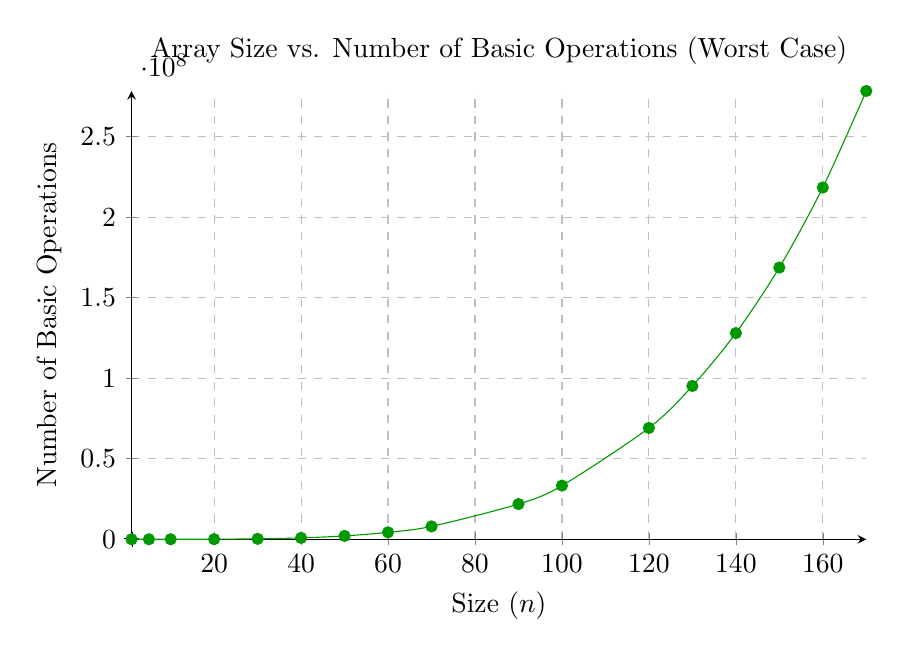
\begin{tikzpicture}
		\begin{axis}[
			% Axis labels and title
			title={Array Size vs. Number of Basic Operations (Worst Case)},
			xlabel={Size (\(n\))},
			ylabel={Number of Basic Operations},
			% Axis limits
			%xmin=0, xmax=100,
			ymin=0, %ymax=200,
			% Axis ticks
			% xtick={0,20,40,60,80,100},
			% ytick={0,20,40,60,80,100,120},
			grid=both,
			axis lines=left,
			axis line style={|-stealth},
			grid style=dashed,
			width=0.9\textwidth,
			height=\axisdefaultheight
			]
			\addplot[
				color=green!60!black,
				mark=*,
				smooth
				]
			% Change the coordinates here with your own data:
			coordinates {
				(1,   2)
				(5,   215)
				(10,  3337)
				(20, 53286)
				(30,  269841)
				(40, 852998)
				(50,  2082757)
				(60,  4319121)
				(70,  8002082)
				(90,  21867815)
				(100, 33330582)
				(120, 69115922)
				(130, 95198487)
				(140, 128047659)
				(150, 168743430)
				(160, 218445802)
				(170, 278394775)
			};
		\end{axis}
	\end{tikzpicture}
	\end{figure}

\subsubsection{Comments}

\begin{itemize}
    \item \textbf{Basic Operation Marked as (1) vs Real Execution Time:} \\
    The theoretical graph for (1) shows a linear relationship with \(n\), which does not align with the real execution graph. Its linear complexity makes it an inappropriate representation of the algorithm’s worst-case behavior.

    \item \textbf{Basic Operation Marked as (2) vs Real Execution Time:} \\
    The theoretical graph for (2) exhibits a complexity of \(n^2\), which grows slower than the real execution graph. This mismatch makes it an invalid choice for modeling the worst case.

    \item \textbf{Basic Operation Marked as (3) vs Real Execution Time:} \\
    The theoretical graph for (3) reflects a complexity of \(n^3\). While it grows faster than \(n^2\), it still does not align well with the real execution graph, making it an unsuitable choice.

    \item \textbf{Basic Operation Marked as (4) vs Real Execution Time:} \\
    The theoretical graph for (4) reflects a complexity of \(n^4\), which closely aligns with the real execution graph. This makes it the most accurate and appropriate choice for representing the algorithm’s worst-case behavior.
\end{itemize}




	\subsection{Average Case}

\subsubsection{Graph of the real execution time of the algorithm}

  \begin{figure}[H]
	\centering
	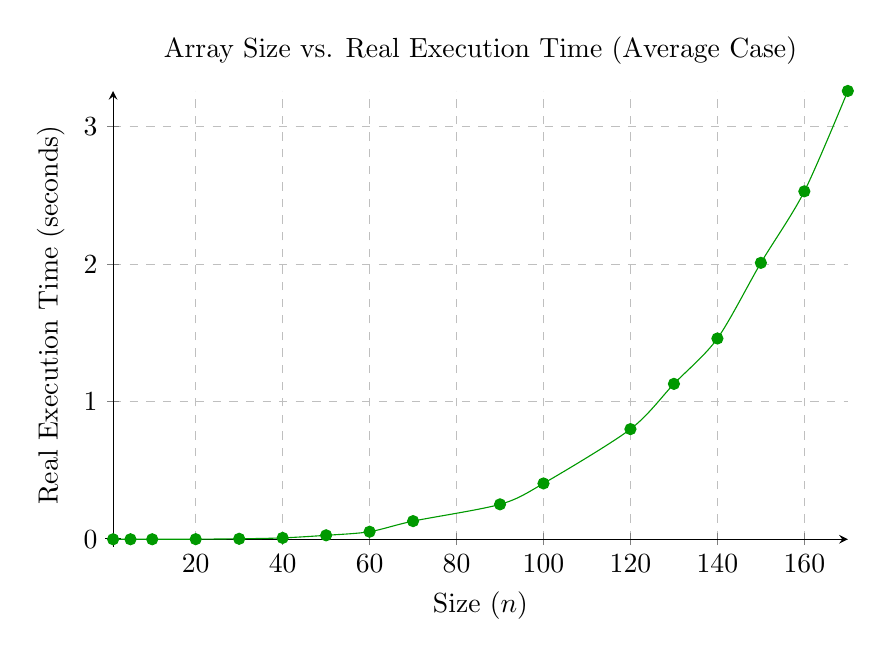
\begin{tikzpicture}
		\begin{axis}[
			% Axis labels and title
			title={Array Size vs. Real Execution Time (Average Case)},
			xlabel={Size (\(n\))},
			ylabel={Real Execution Time (seconds)},
			% Axis limits
			%xmin=0, xmax=100,
			ymin=0, %ymax=200,
			% Axis ticks
			% xtick={0,20,40,60,80,100},
			% ytick={0,20,40,60,80,100,120},
			grid=both,
			axis lines=left,
			axis line style={|-stealth},
			grid style=dashed,
			width=0.9\textwidth,
			height=\axisdefaultheight
			]
			\addplot[
				color=green!60!black,
				mark=*,
				smooth
				]
			% Change the coordinates here with your own data:
			coordinates {
				(1, 0.000000596)
				(5,   0.00000553)
				(10,  0.0000539)
				(20,  0.000734)
				(30,  0.00345)
				(40,  0.00999)
				(50,  0.0288)
				(60,  0.0549)
				(70,  0.132)
				(90,  0.254)
				(100, 0.406)
				(120, 0.801)
				(130, 1.13)
				(140, 1.46)
				(150, 2.01)
				(160, 2.53)
				(170, 3.26)
			};
		\end{axis}
	\end{tikzpicture}
	\end{figure}
	
	\subsubsection{Graph of the theoretical analysis when basic operation is the operation marked as (1)}

 \begin{figure}[H]
	\centering
	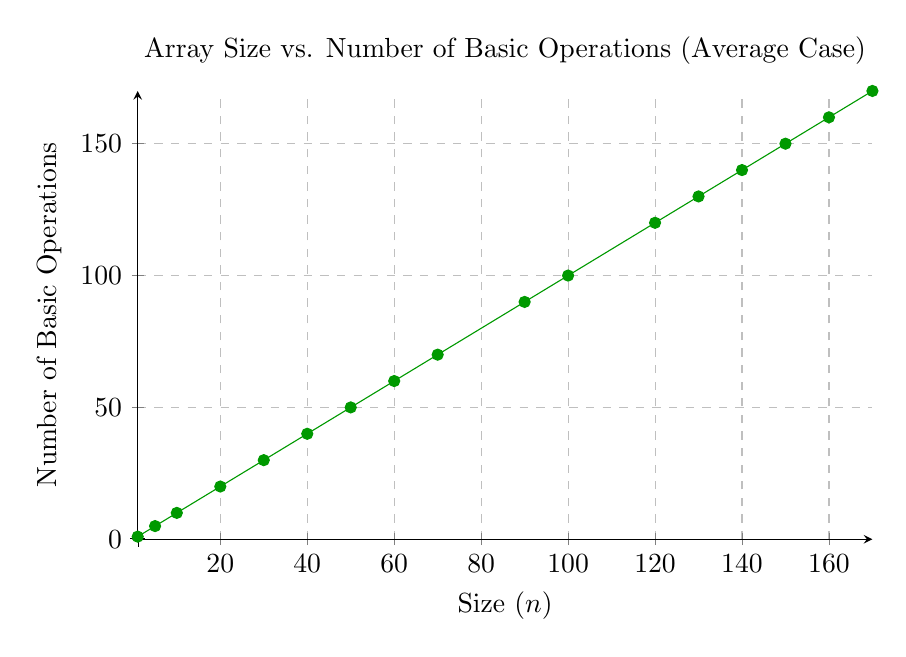
\begin{tikzpicture}
		\begin{axis}[
			% Axis labels and title
			title={Array Size vs. Number of Basic Operations (Average Case)},
			xlabel={Size (\(n\))},
			ylabel={Number of Basic Operations},
			% Axis limits
			%xmin=0, xmax=100,
			ymin=0, %ymax=200,
			% Axis ticks
			% xtick={0,20,40,60,80,100},
			% ytick={0,20,40,60,80,100,120},
			grid=both,
			axis lines=left,
			axis line style={|-stealth},
			grid style=dashed,
			width=0.9\textwidth,
			height=\axisdefaultheight
			]
			\addplot[
				color=green!60!black,
				mark=*,
				smooth
				]
			% Change the coordinates here with your own data:
			coordinates {
				(1,   1)
				(5,   5)
				(10,  10)
				(20, 20)
				(30,  30)
				(40, 40)
				(50,  50)
				(60,  60)
				(70,  70)
				(90,  90)
				(100,100)
				(120, 120)
				(130, 130)
				(140, 140)
				(150, 150)
				(160, 160)
				(170,170)
			};
		\end{axis}
	\end{tikzpicture}
	\end{figure}

	\subsubsection{Graph of the theoretical analysis when basic operation is the operation marked as (2)}

  \begin{figure}[H]
	\centering
	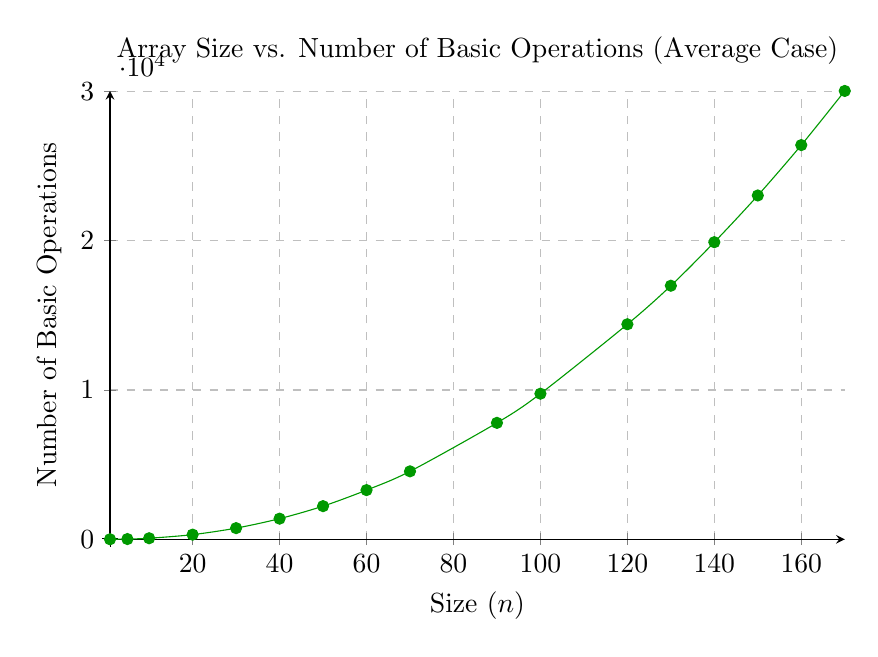
\begin{tikzpicture}
		\begin{axis}[
			% Axis labels and title
			title={Array Size vs. Number of Basic Operations (Average Case)},
			xlabel={Size (\(n\))},
			ylabel={Number of Basic Operations},
			% Axis limits
			%xmin=0, xmax=100,
			ymin=0, %ymax=200,
			% Axis ticks
			% xtick={0,20,40,60,80,100},
			% ytick={0,20,40,60,80,100,120},
			grid=both,
			axis lines=left,
			axis line style={|-stealth},
			grid style=dashed,
			width=0.9\textwidth,
			height=\axisdefaultheight
			]
			\addplot[
				color=green!60!black,
				mark=*,
				smooth
				]
			% Change the coordinates here with your own data:
			coordinates {
				(1,   0.25)
				(5,   14.375)
				(10,  68.75)
				(20, 310)
				(30,  746.25)
				(40, 1380)
				(50,  2218.75)
				(60,  3292.5)
				(70,  4550)
				(90,  7796.25)
				(100,9750)
				(120, 14400)
				(130, 16981.25)
				(140, 19897.5)
				(150, 23025)
				(160, 26400)
				(170,30026.25)
			};
		\end{axis}
	\end{tikzpicture}
	\end{figure}

	\subsubsection{Graph of the theoretical analysis when basic operation is the operation marked as (3)}

  \begin{figure}[H]
	\centering
	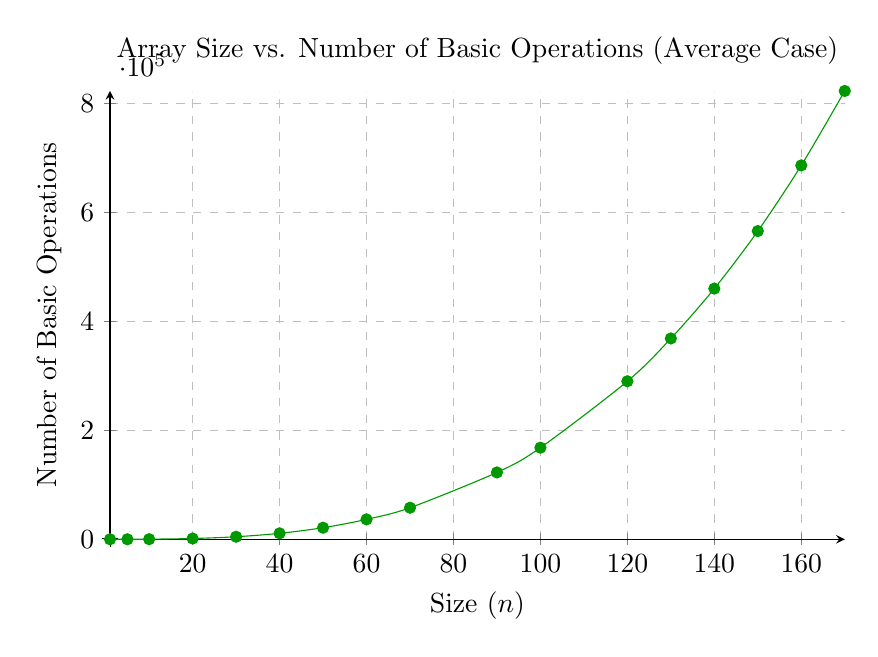
\begin{tikzpicture}
		\begin{axis}[
			% Axis labels and title
			title={Array Size vs. Number of Basic Operations (Average Case)},
			xlabel={Size (\(n\))},
			ylabel={Number of Basic Operations},
			% Axis limits
			%xmin=0, xmax=100,
			ymin=0, %ymax=200,
			% Axis ticks
			% xtick={0,20,40,60,80,100},
			% ytick={0,20,40,60,80,100,120},
			grid=both,
			axis lines=left,
			axis line style={|-stealth},
			grid style=dashed,
			width=0.9\textwidth,
			height=\axisdefaultheight
			]
			\addplot[
				color=green!60!black,
				mark=*,
				smooth
				]
			% Change the coordinates here with your own data:
			coordinates {
				(1,   0.25)
				(5,   28.125)
				(10,  190)
				(20, 1410)
				(30,  4656.25)
				(40, 10935)
				(50,  21231.25)
				(60,  36552.5)
				(70,  57916.25)
				(90,  122688.75)
				(100,168112.5)
				(120, 290035)
				(130, 368582.5)
				(140, 460110)
				(150, 565662.5)
				(160, 686240)
				(170,822842.5)
			};
		\end{axis}
	\end{tikzpicture}
	\end{figure}

	\subsubsection{Graph of the theoretical analysis when basic operation is the operation marked as (4)}

  \begin{figure}[H]
	\centering
	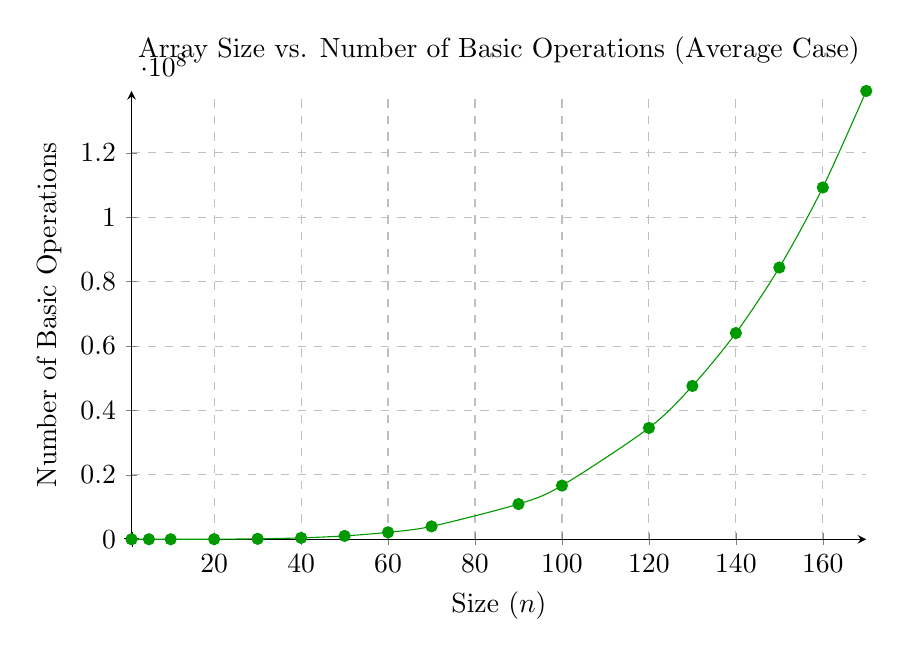
\begin{tikzpicture}
		\begin{axis}[
			% Axis labels and title
			title={Array Size vs. Number of Basic Operations (Average Case)},
			xlabel={Size (\(n\))},
			ylabel={Number of Basic Operations},
			% Axis limits
			%xmin=0, xmax=100,
			ymin=0, %ymax=200,
			% Axis ticks
			% xtick={0,20,40,60,80,100},
			% ytick={0,20,40,60,80,100,120},
			grid=both,
			axis lines=left,
			axis line style={|-stealth},
			grid style=dashed,
			width=0.9\textwidth,
			height=\axisdefaultheight
			]
			\addplot[
				color=green!60!black,
				mark=*,
				smooth
				]
			% Change the coordinates here with your own data:
			coordinates {
				(1,   0.375)
				(5,   114.375)
				(10,  1708.75)
				(20, 26845)
				(30,  135427.5)
				(40, 427465)
				(50,  1042950)
				(60,  2161920)
				(70,  4004341.25)
				(90,  10939635)
				(100,16672487.5)
				(120, 34568685)
				(130, 47611963.75)
				(140, 64038782.5)
				(150, 84389062.5)
				(160, 109242840)
				(170,139220118.75)
			};
		\end{axis}
	\end{tikzpicture}
	\end{figure}



\subsubsection{Comments}

\begin{itemize}
    \item \textbf{Basic Operation Marked as (1) vs Real Execution Time:} \\
    The theoretical graph for (1) shows a linear relationship with \(n\), which does not align with the real execution graph. Its simplicity makes it an inappropriate representation of the algorithm’s average-case behavior.

    \item \textbf{Basic Operation Marked as (2) vs Real Execution Time:} \\
    The theoretical graph for (2) reflects a complexity of \(n^2 \log n\), which grows slower than the real execution graph. This mismatch makes it an unsuitable choice for modeling the average case.

    \item \textbf{Basic Operation Marked as (3) vs Real Execution Time:} \\
    The theoretical graph for (3) reflects a complexity of \(n^3\). While it shows faster growth than \(n^2 \log n\), it still does not align well with the real execution graph, making it an inadequate representation.

    \item \textbf{Basic Operation Marked as (4) vs Real Execution Time:} \\
    The theoretical graph for (4) reflects a complexity of \(n^4\), which closely aligns with the real execution graph. This makes it the most appropriate and realistic choice for representing the algorithm’s average-case behavior.
\end{itemize}

\end{document}
